% Dissertation template for the Champalimaud Neuroscience Programme
%
%   
% Adapted from Princeton University's template
% Author: Jeffrey Scott Dwoskin <jdwoskin@princeton.edu>
% Adapted from: http://www.math.princeton.edu/graduate/tex/puthesis.html
% and
% the template from Universitat Pompeu Fabra, in B5
% http://www.upf.edu/bibtic/en/guiesiajudes/eines/tesis/quart.html#template
% 
% José R Fernandes, January 2015




% ****************************************************************************************** %
% SETTINGS
% 
%%% For print copies
%% set 'singlespace' option to set entire thesis to single space, and define "\printmode" to remove all hyperlinks for printed copies of the thesis. Delete all output files before changing this mode -- it will turn hyperref package on and off
%\documentclass[12pt,lot, lof, singlespace]{puthesis}
%\newcommand{\printmode}{}

%%% For the electronic copy, use doublespacing, define "\proquestmode" to use outlined links, instead of colored links. 
%%% 
%%% ITQB's paper size is B5
%%% 
\documentclass[11pt,lot,lof,b5paper]{puthesis} 
\usepackage[utf8]{inputenc}
\usepackage[T1]{fontenc}
\newcommand{\proquestmode}{}

% I prefer proquestmode to be off for electronic copies for normal use, since the colored links are less distracting. However when printed in black and white, the colored links are difficult to read. 

%%% For early drafts without some of the frontmatter
% Also see the "ifodd" command below to disable more frontmatter
%\documentclass[12pt]{puthesis}




%%%%%%%%%%%%%%%%%%%%%%%%%%%%%%%%%%%%%%%%%%%%%%%%%%%%%%%%%%%%%\
%%%% Author & title page info

\title{Travels into Several Remote Nations of the World. In Four Parts.}
%
\submitted{2015}  % degree conferral date (January, April, June, September, or November)
\copyrightyear{2015}  % year in which the copyright is secured by publication of the dissertation.
\author{Gonçalo C. Lopes}
\adviser{Joseph J. Paton and Adam R. Kampff}  %replace with the full name of your adviser
\departmentprefix{International Neuroscience Doctoral Programme}  % defaults to "Department of", but programs need to change this.
\department{Champalimaud Neuroscience Programme}






%%%%%%%%%%%%%%%%%%%%%%%%%%%%%%%%%%%%%%%%%%%%%%%%%%%%%%%%%%%%%\
%%%% Tweak float placements
% From: http://mintaka.sdsu.edu/GF/bibliog/latex/floats.html "Controlling LaTeX Floats"
% and based on: http://www.tex.ac.uk/cgi-bin/texfaq2html?label=floats
% LaTeX defaults listed at: http://people.cs.uu.nl/piet/floats/node1.html

% Alter some LaTeX defaults for better treatment of figures:
    % See p.105 of "TeX Unbound" for suggested values.
    % See pp. 199-200 of Lamport's "LaTeX" book for details.
    %   General parameters, for ALL pages:
    \renewcommand{\topfraction}{0.85}	% max fraction of floats at top
    \renewcommand{\bottomfraction}{0.6}	% max fraction of floats at bottom
    %   Parameters for TEXT pages (not float pages):
    \setcounter{topnumber}{2}
    \setcounter{bottomnumber}{2}
    \setcounter{totalnumber}{4}     % 2 may work better
    \setcounter{dbltopnumber}{2}    % for 2-column pages
    \renewcommand{\dbltopfraction}{0.66}	% fit big float above 2-col. text
    \renewcommand{\textfraction}{0.15}	% allow minimal text w. figs
    %   Parameters for FLOAT pages (not text pages):
    \renewcommand{\floatpagefraction}{0.66}	% require fuller float pages
	% N.B.: floatpagefraction MUST be less than topfraction !!
    \renewcommand{\dblfloatpagefraction}{0.66}	% require fuller float pages

% The documentclass already sets parameters to make a high penalty for widows and orphans. 



%%%%%%%%%%%%%%%%%%%%%%%%%%%%%%%%%%%%%%%%%%%%%%%%%%%%%%%%%%%%%\
%%% Printed vs. online formatting
\ifdefined\printmode

% Printed copy
% url package understands urls (with proper line-breaks) without hyperlinking them
\usepackage{url}

\else

\ifdefined\proquestmode
%ProQuest copy -- http://www.princeton.edu/~mudd/thesis/Submissionguide.pdf

% ProQuest requires a double spaced version (set previously). They will take an electronic copy, so we want links in the pdf, but also copies may be printed or made into microfilm in black and white, so we want outlined links instead of colored links.
\usepackage[hidelinks]{hyperref}
\hypersetup{bookmarksnumbered}

% copy the already-set title and author to use in the pdf properties
\makeatletter
\hypersetup{pdftitle=\@title,pdfauthor=\@author}
\makeatother

\else
% Online copy

% adds internal linked references, pdf bookmarks, etc

% turn all references and citations into hyperlinks:
%  -- not for printed copies
% -- automatically includes url package
% options:
%   colorlinks makes links by coloring the text instead of putting a rectangle around the text.
\usepackage[hidelinks]{hyperref}
\hypersetup{colorlinks,bookmarksnumbered}


% make the page number rather than the text be the link for ToC entries
%\hypersetup{linktocpage}
\fi % proquest or online formatting
\fi % printed or online formatting


%%%%%%%%%%%%%%%%%%%%%%%%%%%%%%%%%%%%%%%%%%%%%%%%%%%%%%%%%%%%%\
%%%% Use packages 
%%%% 
%%%% add any extra packages you need

%\usepackage{amsfonts}

%%% For figures
\usepackage{graphicx}
\DeclareGraphicsExtensions{.pdf,.png,.jpg}
%\usepackage{subfig,rotate}

%%% for inline lists
\usepackage{paralist}

%%% for comments
\usepackage{verbatim}

%%% For tables
\usepackage{multirow}
\usepackage[table]{xcolor}

% Longtable lets you have tables that span multiple pages.
\usepackage{longtable}
\usepackage{pdflscape}
\usepackage{afterpage}
\usepackage{geometry}

% Booktabs produces far nicer tables than the standard LaTeX tables.
%   see: http://en.wikibooks.org/wiki/LaTeX/Tables
\usepackage{pdfpages}
\usepackage{booktabs}

%set parameters for longtable:
% default caption width is 4in for longtable, but wider for normal tables
\setlength{\LTcapwidth}{\textwidth}

%bibliography packages
\usepackage[]{apacite}

%\setcitestyle{authoryear,round,semicolon,aysep={},yysep={,}}

%math packages
\usepackage{amsmath, amsthm, amssymb}
\usepackage{amssymb}

%specifying table and figure packages
\usepackage{sidecap}
\usepackage{multirow}
\usepackage[labelfont=it,labelsep=period]{caption}

%%%% Define commands

% Define any custom commands that you want to use.
% For example, highlight notes for future edits to the thesis
%\newcommand{\todo}[1]{\textbf{\emph{TODO:}#1}}

% create an environment that will indent text
% see: http://latex.computersci.org/Reference/ListEnvironments
% 	\raggedright makes them left aligned instead of justified
\newenvironment{indenttext}{
    \begin{list}{}{ \itemsep 0in \itemindent 0in
    \labelsep 0in \labelwidth 0in
    \listparindent 0in
    \topsep 0in \partopsep 0in \parskip 0in \parsep 0in
    \leftmargin 1em \rightmargin 0in
    \raggedright
    }
    \item
  }
  {\end{list}}

% another environment that's an indented list, with no spaces between items -- if we want multiple items/lines. Useful in tables. Use \item inside the environment.
% 	\raggedright makes them left aligned instead of justified
\newenvironment{indentlist}{
    \begin{list}{}{ \itemsep 0in \itemindent 0in
    \labelsep 0in \labelwidth 0in
    \listparindent 0in
    \topsep 0in \partopsep 0in \parskip 0in \parsep 0in
    \leftmargin 1em \rightmargin 0in
    \raggedright
    }

  }
  {\end{list}}

%set exceptions for hyphenation


%%%%%%%%%%%%%%%%%%%%%%%%%%%%%%%%%%%%%%%%%%%%%%%%%%%%%%%%%%%%%\
%%%% Front-matter

% For early drafts, you may want to disable some of the frontmatter. Simply change this to "\ifodd 1" to do so.
\ifodd 0
%% front-matter disabled while writing chapters
\renewcommand{\maketitlepage}{}
\renewcommand*{\makecopyrightpage}{}
\renewcommand*{\makeabstract}{}
%
%% you can just skip the \acknowledgements and \dedication commands to leave out these sections.
%
\else
%
%
\dedication{% !TEX root = ../Thesis_Sep_2013.tex


\label{dedication}


\emph{To ?}}
\acknowledgments{% !TEX root = ../Thesis_Sep_2013.tex


\label{acknow}

I hope you will be ready to own publicly, whenever you shall be called to it, that by your great and frequent urgency you prevailed on me to publish a very loose and uncorrect account of my travels, with directions to hire some young gentleman of either university to put them in order, and correct the style, as my cousin Dampier did, by my advice, in his book called “A Voyage round the world.”  But I do not remember I gave you power to consent that any thing should be omitted, and much less that any thing should be inserted; therefore, as to the latter, I do here renounce every thing of that kind; particularly a paragraph about her majesty Queen Anne, of most pious and glorious memory; although I did reverence and esteem her more than any of human species.  But you, or your interpolator, ought to have considered, that it was not my inclination, so was it not decent to praise any animal of our composition before my master Houyhnhnm: And besides, the fact was altogether false; for to my knowledge, being in England during some part of her majesty’s reign, she did govern by a chief minister; nay even by two successively, the first whereof was the lord of Godolphin, and the second the lord of Oxford; so that you have made me say the thing that was not.  Likewise in the account of the academy of projectors, and several passages of my discourse to my master Houyhnhnm, you have either omitted some material circumstances, or minced or changed them in such a manner, that I do hardly know my own work.  When I formerly hinted to you something of this in a letter, you were pleased to answer that you were afraid of giving offence; that people in power were very watchful over the press, and apt not only to interpret, but to punish every thing which looked like an innuendo (as I think you call it).  But, pray how could that which I spoke so many years ago, and at about five thousand leagues distance, in another reign, be applied to any of the Yahoos, who now are said to govern the herd; especially at a time when I little thought, or feared, the unhappiness of living under them?  Have not I the most reason to complain, when I see these very Yahoos carried by Houyhnhnms in a vehicle, as if they were brutes, and those the rational creatures?  And indeed to avoid so monstrous and detestable a sight was one principal motive of my retirement hither.

Thus much I thought proper to tell you in relation to yourself, and to the trust I reposed in you.

I do, in the next place, complain of my own great want of judgment, in being prevailed upon by the entreaties and false reasoning of you and some others, very much against my own opinion, to suffer my travels to be published.  Pray bring to your mind how often I desired you to consider, when you insisted on the motive of public good, that the Yahoos were a species of animals utterly incapable of amendment by precept or example: and so it has proved; for, instead of seeing a full stop put to all abuses and corruptions, at least in this little island, as I had reason to expect; behold, after above six months warning, I cannot learn that my book has produced one single effect according to my intentions.  I desired you would let me know, by a letter, when party and faction were extinguished; judges learned and upright; pleaders honest and modest, with some tincture of common sense, and Smithfield blazing with pyramids of law books; the young nobility’s education entirely changed; the physicians banished; the female Yahoos abounding in virtue, honour, truth, and good sense; courts and levees of great ministers thoroughly weeded and swept; wit, merit, and learning rewarded; all disgracers of the press in prose and verse condemned to eat nothing but their own cotton, and quench their thirst with their own ink.  These, and a thousand other reformations, I firmly counted upon by your encouragement; as indeed they were plainly deducible from the precepts delivered in my book.  And it must be owned, that seven months were a sufficient time to correct every vice and folly to which Yahoos are subject, if their natures had been capable of the least disposition to virtue or wisdom.  Yet, so far have you been from answering my expectation in any of your letters; that on the contrary you are loading our carrier every week with libels, and keys, and reflections, and memoirs, and second parts; wherein I see myself accused of reflecting upon great state folk; of degrading human nature (for so they have still the confidence to style it), and of abusing the female sex.  I find likewise that the writers of those bundles are not agreed among themselves; for some of them will not allow me to be the author of my own travels; and others make me author of books to which I am wholly a stranger.

I find likewise that your printer has been so careless as to confound the times, and mistake the dates, of my several voyages and returns; neither assigning the true year, nor the true month, nor day of the month: and I hear the original manuscript is all destroyed since the publication of my book; neither have I any copy left: however, I have sent you some corrections, which you may insert, if ever there should be a second edition: and yet I cannot stand to them; but shall leave that matter to my judicious and candid readers to adjust it as they please.

I hear some of our sea Yahoos find fault with my sea-language, as not proper in many parts, nor now in use.  I cannot help it.  In my first voyages, while I was young, I was instructed by the oldest mariners, and learned to speak as they did.  But I have since found that the sea Yahoos are apt, like the land ones, to become new-fangled in their words, which the latter change every year; insomuch, as I remember upon each return to my own country their old dialect was so altered, that I could hardly understand the new.  And I observe, when any Yahoo comes from London out of curiosity to visit me at my house, we neither of us are able to deliver our conceptions in a manner intelligible to the other.

If the censure of the Yahoos could any way affect me, I should have great reason to complain, that some of them are so bold as to think my book of travels a mere fiction out of mine own brain, and have gone so far as to drop hints, that the Houyhnhnms and Yahoos have no more existence than the inhabitants of Utopia.

Indeed I must confess, that as to the people of Lilliput, Brobdingrag (for so the word should have been spelt, and not erroneously Brobdingnag), and Laputa, I have never yet heard of any Yahoo so presumptuous as to dispute their being, or the facts I have related concerning them; because the truth immediately strikes every reader with conviction.  And is there less probability in my account of the Houyhnhnms or Yahoos, when it is manifest as to the latter, there are so many thousands even in this country, who only differ from their brother brutes in Houyhnhnmland, because they use a sort of jabber, and do not go naked?  I wrote for their amendment, and not their approbation.  The united praise of the whole race would be of less consequence to me, than the neighing of those two degenerate Houyhnhnms I keep in my stable; because from these, degenerate as they are, I still improve in some virtues without any mixture of vice.

Do these miserable animals presume to think, that I am so degenerated as to defend my veracity?  Yahoo as I am, it is well known through all Houyhnhnmland, that, by the instructions and example of my illustrious master, I was able in the compass of two years (although I confess with the utmost difficulty) to remove that infernal habit of lying, shuffling, deceiving, and equivocating, so deeply rooted in the very souls of all my species; especially the Europeans.

I have other complaints to make upon this vexatious occasion; but I forbear troubling myself or you any further.  I must freely confess, that since my last return, some corruptions of my Yahoo nature have revived in me by conversing with a few of your species, and particularly those of my own family, by an unavoidable necessity; else I should never have attempted so absurd a project as that of reforming the Yahoo race in this kingdom: But I have now done with all such visionary schemes for ever.


   
   

}
\abstract{\label{ch:abstract}

The function of mammalian motor cortex has been a persistent mystery. There is a long history of research linking activity in this part of the brain with the control of ``voluntary'' movements but surprisingly there is an equally large body of evidence in non-human animals describing all kinds of complex behaviours that are \emph{not} impaired when motor cortex is fully removed. What is the reason behind this discrepancy? What kind of movements are actually controlled by motor cortex? This thesis attempts to reconcile the many conflicting views on the cortical control of movement and outline a strategy for investigating the teleology of this brain region.

We start out by introducing a new set of hardware and software tools for neuroscience that aim to make it easier to study in detail more naturalistic motor behaviours in rodents. These tools allow the experimenter to quickly reconfigure the physical and virtual environment of a behaviour task while simultaneously tracking in real-time fine-scale measurements of motor performance.

We then set out to investigate the behaviour of rats facing unexpected or unpredictable motor challenges while navigating dynamic obstacle courses with or without motor cortex. Surprisingly, we found that rats without motor cortex show visible impairments when dealing for the first time with an unexpected motor challenge, despite retaining the ability to skilfully adapt to the new environment with repeated trials.

This observation has led us to propose and discuss a primordial role for motor cortex in extending the robustness of sub-cortical movement systems. Specifically, we suggest that motor cortex is the structure that has helped mammals to conquer those situations that require a succession of rapid and adapted behavioural responses to unexpected environmental change; the kind of resourcefulness that is one of the defining characteristics of mammalian phylogeny.
}
\abstractport{\label{ch:abstractPT}

%\hyphenation{co-nhe-ci-men-to,par-ti-ci-pan-tes}

\begin{center}
\Large \textbf{T\'{i}tulo}
\end{center}

Uma Função Robusta para o Córtex Motor

\begin{center}
\Large \textbf{Resumo}
\end{center}

A determinação da função exacta do córtex motor existente no cérebro dos mamíferos tem sido um mistério que persistiu ao longo do tempo. Existe uma longa história de estudos que ligam a actividade desta área do cérebro ao controlo de movimentos ``voluntários'' mas, curiosamente, existe uma história igualmente longa de estudos em animais descrevendo uma grande variedade de movimentos complexos que \emph{não são} afectados com a remoção total do córtex motor. Qual a razão por detrás desta discrepância? Que tipo de movimentos serão realmente controlados pelo córtex motor? Esta tese procura reconciliar as muitas perspectivas existentes sobre o controlo do córtex sobre os movimentos e sugerir uma estratégia para investigar a teleologia desta região do cérebro.

Começamos por introduzir um conjunto de ferramentas de \emph{hardware} e \emph{software} para facilitar o estudo detalhado de comportamentos motores em situações naturalistas em roedores. Estas ferramentas permitem ao cientista reconfigurar rapidamente o contexto físico e lógico de uma tarefa comportamental em simultâneo com a medição precisa e em tempo-real de vários parâmetros de performance motora.

De seguida investigamos o comportamento de ratos, com e sem o córtex motor, durante a travessia de um percurso de obstáculos em que eram apresentados novos desafios motores inesperados. Surpreendentemente, observámos que os ratos em que o córtex motor havia sido removido demonstraram dificuldade em lidar pela primeira vez com um desafio motor inesperado, apesar de preservarem a sua capacidade de se adaptar com eficácia ao novo ambiente após sucessivas tentativas.

Esta observação levou-nos a propor e discutir uma possível função primordial para o córtex motor: estender a robustez dos sistemas sub-corticais responsáveis pelo controlo dos movimentos. Especificamente, sugerimos que o córtex motor é a estrutura que permite aos mamíferos ultrapassar situações que requerem uma sucessão de respostas comportamentais rápidas e adaptadas a um novo contexto; uma das capacidades que reconhecemos como característica do reino mamífero.
}
\contrib{\input{chapters/authorcontrib}}


%%%%%%%%%%%%%%%%%%%%%%%%%%%%%%%%%%%%%%%%%%%%%%%%%%%%%%%%%%%%%\
%%%% Hide some chapters

%%% If you want to produce a pdf that includes only certain chapters, specify them with includeonly, in addition to including all chapters below.
%\includeonly{ch-intro/chapter-intro}
%%% You can also specify multiple chapters.
%\includeonly{ch-intro/chapter-intro,ch-usage/chapter-usage}
%\includeonly{chap1,chap2,chap3}


%%%%%%%%%%%%%%%%%%%%%%%%%%%%%%%%%%%%%%%%%%%%%%%%%%%%%%%%%%%%%
%%%% Notes:

% Footnotes should be placed after punctuation.\footnote{place here.}
% Generally, place citations before the period~\cite{anotherauthor}.
% The proper usage for i.e., and e.g., include commas ``(e.g., option A, option B)''

%%%%%%%%%%%%%%%%%%%%%%%%%%%%%%%%%%%%%%%%%%%%%%%%%%%%%%%%%%%%%

\begin{document}

% % ITQB cover
% 
% Files can be edited in Illustrator
% 
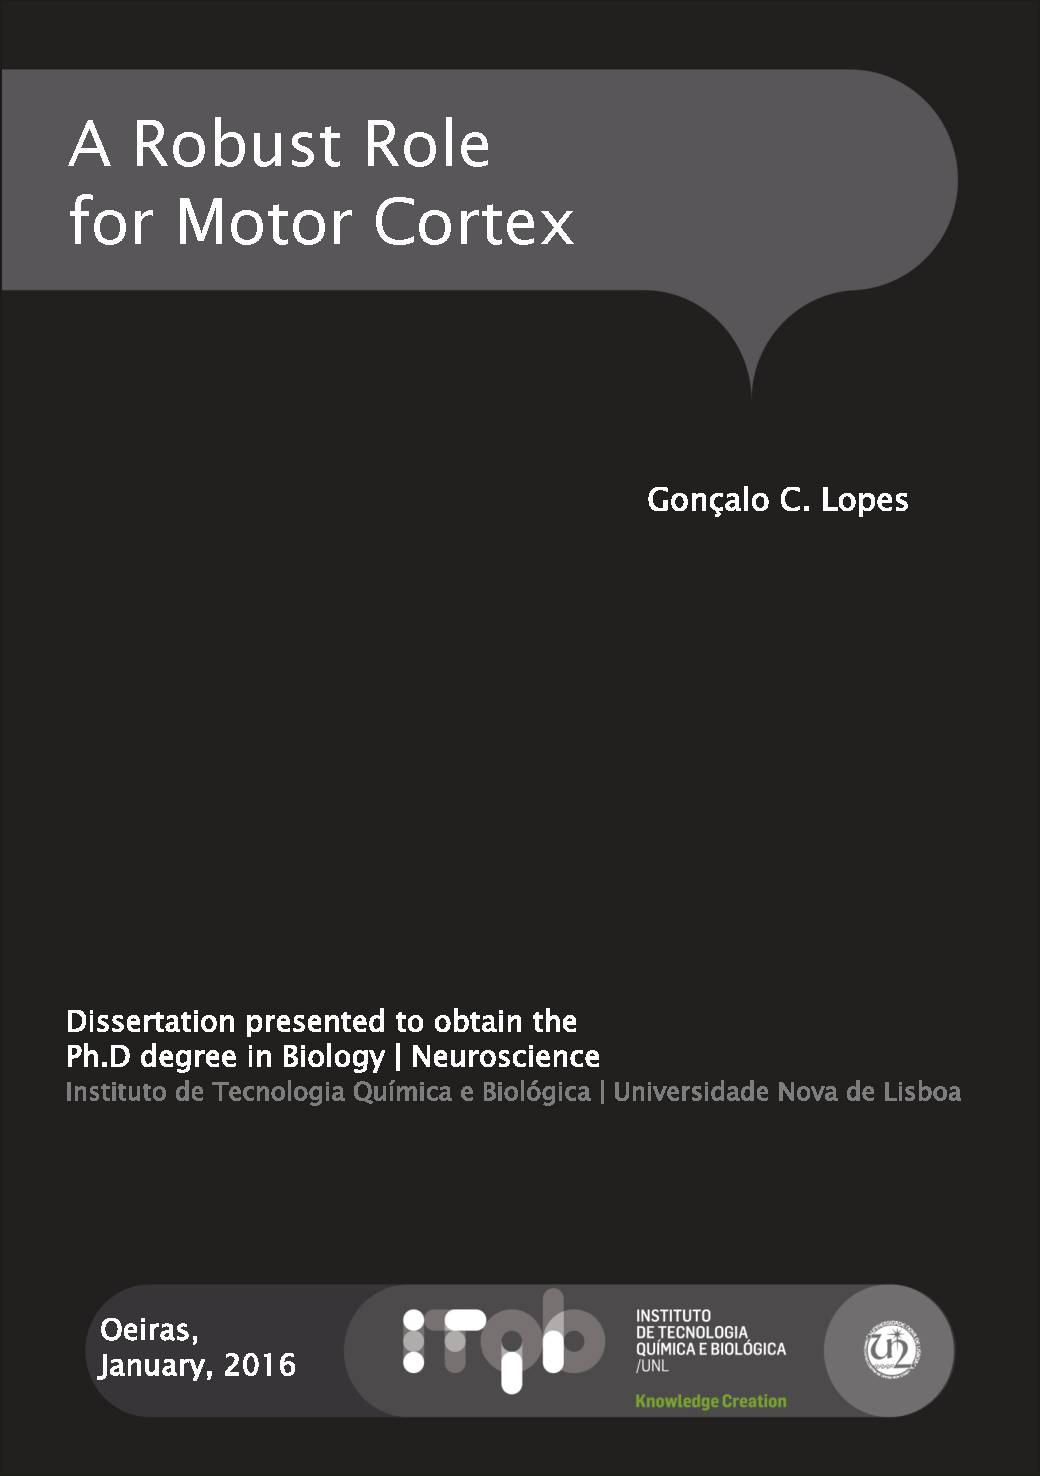
\includepdf[pages={1}]{chapters/Cover.pdf}
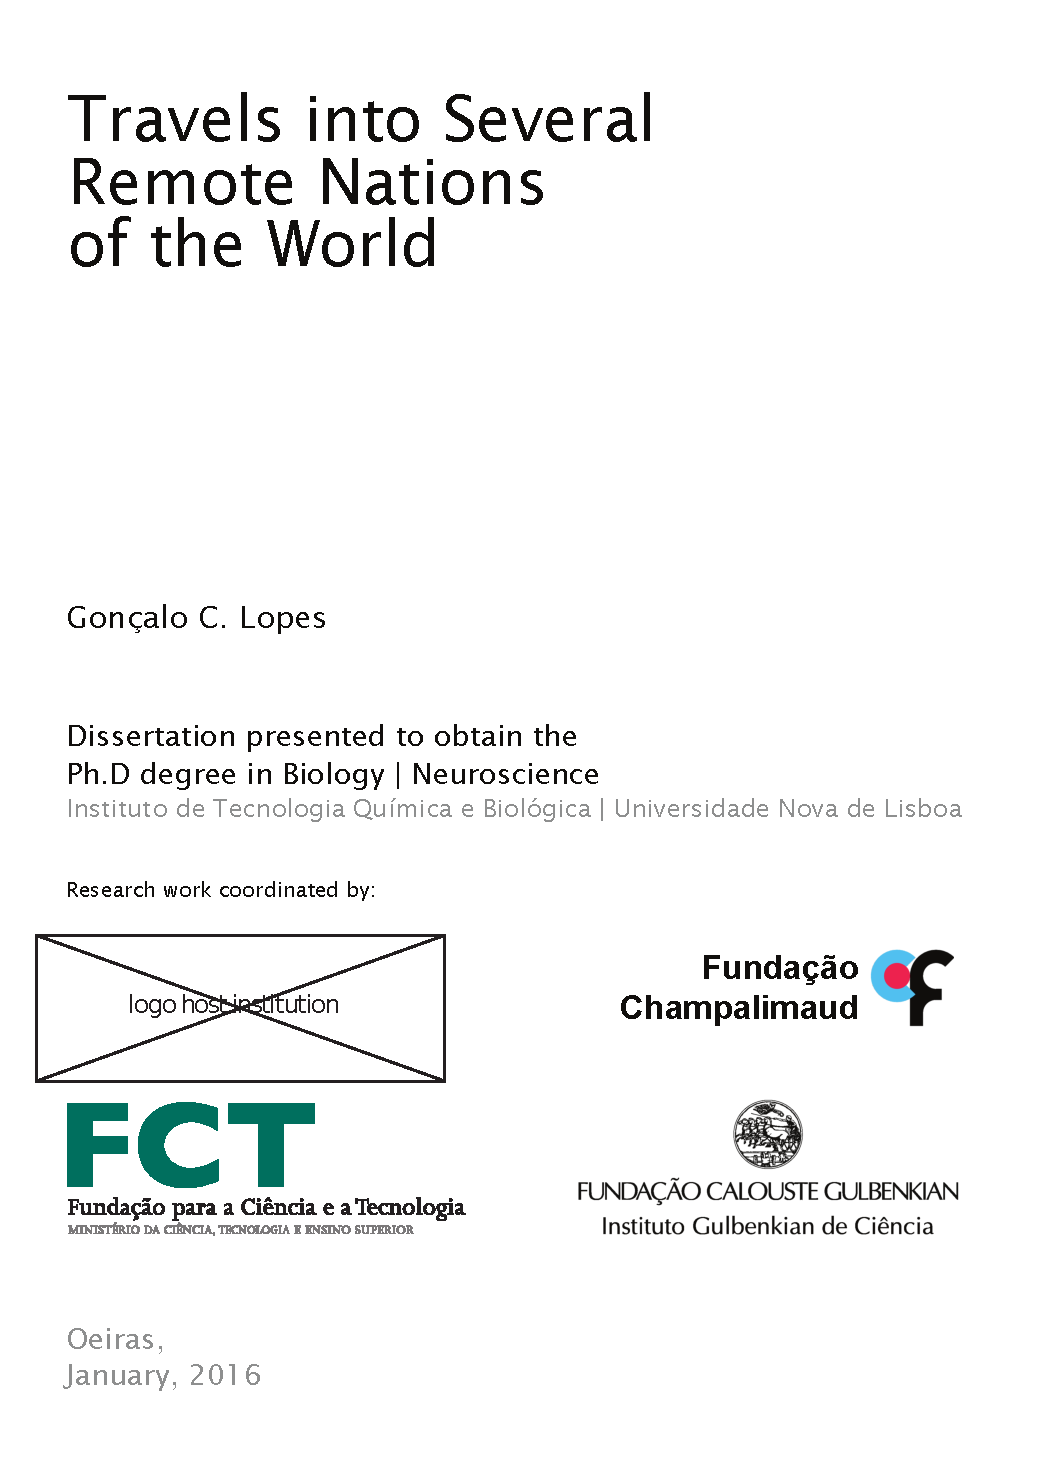
\includepdf[pages={1}]{chapters/TitlePage.pdf}

\maketitlepage
\makefrontmatter

% If you've disabled frontmatter, you can insert the toc manually
\tableofcontents\clearpage

%%%% %%%% Import chapters
%\include lets  us split up the document (and each include starts a new page):

\chapter{Visit to the Academy of Lagado}
				
% !TEX root = ../ThesisTemplateCNP.tex
	

% Chapter summary
				
\section{Chapter Summary}

The author permitted to see the grand academy of Lagado.  The academy largely described.  The arts wherein the professors employ themselves.

\pagebreak




% Visit to Lagado
\section{Visit to the Academy of Lagado}

This academy is not an entire single building, but a continuation of several houses on both sides of a street, which growing waste, was purchased and applied to that use.


I was received very kindly by the warden, and went for many days to the academy.  Every room has in it one or more projectors; and I believe I could not be in fewer than five hundred rooms.

The first man I saw was of a meagre aspect, with sooty hands and face, his hair and beard long, ragged, and singed in several places.  His clothes, shirt, and skin, were all of the same colour.  He has been eight years upon a project for extracting sunbeams out of cucumbers, which were to be put in phials hermetically sealed, and let out to warm the air in raw inclement summers.  He told me, he did not doubt, that, in eight years more, he should be able to supply the governor’s gardens with sunshine, at a reasonable rate: but he complained that his stock was low, and entreated me “to give him something as an encouragement to ingenuity, especially since this had been a very dear season for cucumbers.”  I made him a small present, for my lord had furnished me with money on purpose, because he knew their practice of begging from all who go to see them.

I went into another chamber, but was ready to hasten back, being almost overcome with a horrible stink.  My conductor pressed me forward, conjuring me in a whisper “to give no offence, which would be highly resented;” and therefore I durst not so much as stop my nose.  The projector of this cell was the most ancient student of the academy; his face and beard were of a pale yellow; his hands and clothes daubed over with filth.  When I was presented to him, he gave me a close embrace, a compliment I could well have excused.  His employment, from his first coming into the academy, was an operation to reduce human excrement to its original food, by separating the several parts, removing the tincture which it receives from the gall, making the odour exhale, and scumming off the saliva.  He had a weekly allowance, from the society, of a vessel filled with human ordure, about the bigness of a Bristol barrel.

I saw another at work to calcine ice into gunpowder; who likewise showed me a treatise he had written concerning the malleability of fire, which he intended to publish.

There was a most ingenious architect, who had contrived a new method for building houses, by beginning at the roof, and working downward to the foundation; which he justified to me, by the like practice of those two prudent insects, the bee and the spider.

There was a man born blind, who had several apprentices in his own condition: their employment was to mix colours for painters, which their master taught them to distinguish by feeling and smelling.  It was indeed my misfortune to find them at that time not very perfect in their lessons, and the professor himself happened to be generally mistaken.  This artist is much encouraged and esteemed by the whole fraternity.

In another apartment I was highly pleased with a projector who had found a device of ploughing the ground with hogs, to save the charges of ploughs, cattle, and labour.  The method is this: in an acre of ground you bury, at six inches distance and eight deep, a quantity of acorns, dates, chestnuts, and other mast or vegetables, whereof these animals are fondest; then you drive six hundred or more of them into the field, where, in a few days, they will root up the whole ground in search of their food, and make it fit for sowing, at the same time manuring it with their dung: it is true, upon experiment, they found the charge and trouble very great, and they had little or no crop.  However it is not doubted, that this invention may be capable of great improvement.

I went into another room, where the walls and ceiling were all hung round with cobwebs, except a narrow passage for the artist to go in and out.  At my entrance, he called aloud to me, “not to disturb his webs.”  He lamented “the fatal mistake the world had been so long in, of using silkworms, while we had such plenty of domestic insects who infinitely excelled the former, because they understood how to weave, as well as spin.”  And he proposed further, “that by employing spiders, the charge of dyeing silks should be wholly saved;” whereof I was fully convinced, when he showed me a vast number of flies most beautifully coloured, wherewith he fed his spiders, assuring us “that the webs would take a tincture from them; and as he had them of all hues, he hoped to fit everybody’s fancy, as soon as he could find proper food for the flies, of certain gums, oils, and other glutinous matter, to give a strength and consistence to the threads.”

There was an astronomer, who had undertaken to place a sun-dial upon the great weathercock on the town-house, by adjusting the annual and diurnal motions of the earth and sun, so as to answer and coincide with all accidental turnings of the wind.

I was complaining of a small fit of the colic, upon which my conductor led me into a room where a great physician resided, who was famous for curing that disease, by contrary operations from the same instrument.  He had a large pair of bellows, with a long slender muzzle of ivory: this he conveyed eight inches up the anus, and drawing in the wind, he affirmed he could make the guts as lank as a dried bladder.  But when the disease was more stubborn and violent, he let in the muzzle while the bellows were full of wind, which he discharged into the body of the patient; then withdrew the instrument to replenish it, clapping his thumb strongly against the orifice of then fundament; and this being repeated three or four times, the adventitious wind would rush out, bringing the noxious along with it, (like water put into a pump), and the patient recovered.  I saw him try both experiments upon a dog, but could not discern any effect from the former.  After the latter the animal was ready to burst, and made so violent a discharge as was very offensive to me and my companion.  The dog died on the spot, and we left the doctor endeavouring to recover him, by the same operation.

I visited many other apartments, but shall not trouble my reader with all the curiosities I observed, being studious of brevity.

I had hitherto seen only one side of the academy, the other being appropriated to the advancers of speculative learning, of whom I shall say something, when I have mentioned one illustrious person more, who is called among them “the universal artist.”  He told us “he had been thirty years employing his thoughts for the improvement of human life.”  He had two large rooms full of wonderful curiosities, and fifty men at work.  Some were condensing air into a dry tangible substance, by extracting the nitre, and letting the aqueous or fluid particles percolate; others softening marble, for pillows and pin-cushions; others petrifying the hoofs of a living horse, to preserve them from foundering.  The artist himself was at that time busy upon two great designs; the first, to sow land with chaff, wherein he affirmed the true seminal virtue to be contained, as he demonstrated by several experiments, which I was not skilful enough to comprehend.  The other was, by a certain composition of gums, minerals, and vegetables, outwardly applied, to prevent the growth of wool upon two young lambs; and he hoped, in a reasonable time to propagate the breed of naked sheep, all over the kingdom.

We crossed a walk to the other part of the academy, where, as I have already said, the projectors in speculative learning resided.

The first professor I saw, was in a very large room, with forty pupils about him.  After salutation, observing me to look earnestly upon a frame, which took up the greatest part of both the length and breadth of the room, he said, “Perhaps I might wonder to see him employed in a project for improving speculative knowledge, by practical and mechanical operations.  But the world would soon be sensible of its usefulness; and he flattered himself, that a more noble, exalted thought never sprang in any other man’s head.  Every one knew how laborious the usual method is of attaining to arts and sciences; whereas, by his contrivance, the most ignorant person, at a reasonable charge, and with a little bodily labour, might write books in philosophy, poetry, politics, laws, mathematics, and theology, without the least assistance from genius or study.”  He then led me to the frame, about the sides, whereof all his pupils stood in ranks.  It was twenty feet square, placed in the middle of the room.  The superfices was composed of several bits of wood, about the bigness of a die, but some larger than others.  They were all linked together by slender wires.  These bits of wood were covered, on every square, with paper pasted on them; and on these papers were written all the words of their language, in their several moods, tenses, and declensions; but without any order.  The professor then desired me “to observe; for he was going to set his engine at work.”  The pupils, at his command, took each of them hold of an iron handle, whereof there were forty fixed round the edges of the frame; and giving them a sudden turn, the whole disposition of the words was entirely changed.  He then commanded six-and-thirty of the lads, to read the several lines softly, as they appeared upon the frame; and where they found three or four words together that might make part of a sentence, they dictated to the four remaining boys, who were scribes.  This work was repeated three or four times, and at every turn, the engine was so contrived, that the words shifted into new places, as the square bits of wood moved upside down.


Six hours a day the young students were employed in this labour; and the professor showed me several volumes in large folio, already collected, of broken sentences, which he intended to piece together, and out of those rich materials, to give the world a complete body of all arts and sciences; which, however, might be still improved, and much expedited, if the public would raise a fund for making and employing five hundred such frames in Lagado, and oblige the managers to contribute in common their several collections.

He assured me “that this invention had employed all his thoughts from his youth; that he had emptied the whole vocabulary into his frame, and made the strictest computation of the general proportion there is in books between the numbers of particles, nouns, and verbs, and other parts of speech.”

I made my humblest acknowledgment to this illustrious person, for his great communicativeness; and promised, “if ever I had the good fortune to return to my native country, that I would do him justice, as the sole inventor of this wonderful machine;” the form and contrivance of which I desired leave to delineate on paper, as in the figure here annexed.  I told him, “although it were the custom of our learned in Europe to steal inventions from each other, who had thereby at least this advantage, that it became a controversy which was the right owner; yet I would take such caution, that he should have the honour entire, without a rival.”

We next went to the school of languages, where three professors sat in consultation upon improving that of their own country.

The first project was, to shorten discourse, by cutting polysyllables into one, and leaving out verbs and participles, because, in reality, all things imaginable are but norms.

The other project was, a scheme for entirely abolishing all words whatsoever; and this was urged as a great advantage in point of health, as well as brevity.  For it is plain, that every word we speak is, in some degree, a diminution of our lunge by corrosion, and, consequently, contributes to the shortening of our lives.  An expedient was therefore offered, “that since words are only names for things, it would be more convenient for all men to carry about them such things as were necessary to express a particular business they are to discourse on.”  And this invention would certainly have taken place, to the great ease as well as health of the subject, if the women, in conjunction with the vulgar and illiterate, had not threatened to raise a rebellion unless they might be allowed the liberty to speak with their tongues, after the manner of their forefathers; such constant irreconcilable enemies to science are the common people.  However, many of the most learned and wise adhere to the new scheme of expressing themselves by things; which has only this inconvenience attending it, that if a man’s business be very great, and of various kinds, he must be obliged, in proportion, to carry a greater bundle of things upon his back, unless he can afford one or two strong servants to attend him.  I have often beheld two of those sages almost sinking under the weight of their packs, like pedlars among us, who, when they met in the street, would lay down their loads, open their sacks, and hold conversation for an hour together; then put up their implements, help each other to resume their burdens, and take their leave.

But for short conversations, a man may carry implements in his pockets, and under his arms, enough to supply him; and in his house, he cannot be at a loss.  Therefore the room where company meet who practise this art, is full of all things, ready at hand, requisite to furnish matter for this kind of artificial converse.

Another great advantage proposed by this invention was, that it would serve as a universal language, to be understood in all civilised nations, whose goods and utensils are generally of the same kind, or nearly resembling, so that their uses might easily be comprehended.  And thus ambassadors would be qualified to treat with foreign princes, or ministers of state, to whose tongues they were utter strangers.

I was at the mathematical school, where the master taught his pupils after a method scarce imaginable to us in Europe.  The proposition, and demonstration, were fairly written on a thin wafer, with ink composed of a cephalic tincture.  This, the student was to swallow upon a fasting stomach, and for three days following, eat nothing but bread and water.  As the wafer digested, the tincture mounted to his brain, bearing the proposition along with it.  But the success has not hitherto been answerable, partly by some error in the quantum or composition, and partly by the perverseness of lads, to whom this bolus is so nauseous, that they generally steal aside, and discharge it upwards, before it can operate; neither have they been yet persuaded to use so long an abstinence, as the prescription requires.





%\appendix % all chapters following will be labeled as appendices
%\chapter{Implementation Details\label{ch:implementation}}

Appendices are just chapters, included after the $\backslash appendix$ command.

\section{Switching Formats}
When switching \texttt{printmode} on and off (see Section~\ref{sec:usage:options}), you may need to delete the output .aux files to get the document code to compile correctly. This is because the hyperref package is switched off for \texttt{printmode}, but this package inserts extra tags into the contents lines in the auxiliary files for PDF links, and these can cause errors when the package is not used.

\section{Long Tables}

Long tables span multiple pages. By default they are treated like body text, but we want them to be single spaced all the time. The class therefore defines a new command, $\backslash tablespacing$, that is placed before a long table to switch to single spacing when the rest of the document is in double spacing mode. Another command, $\backslash bodyspacing$, is placed after the long table to switch back to double spacing. Normal tables using \texttt{tabular} automatically use single spacing and do not require the extra commands.

When the documentclass is defined with the `singlespace' option, these commands are automatically adjusted to stay in single spacing after the long table.

Make sure there is always at least one blank line after the $\backslash bodyspacing$ command before the end of the file.

Some times long tables do not format correctly on the first pass. If the column widths are wrong, try running the \LaTeX compiler one or two extra times to allow it to better calculate the column widths.

If you want your long table to break pages at a specific point, you can insert the command $\backslash pagebreak[4]$, to tell \LaTeX that it really should put a page break there. $\backslash pagebreak[2]$ gives it a hint that this is a good place for a page break, if needed. If there's a row that really should not be broken across a page, use $\backslash \backslash *$, which will usually prevent a pagebreak. 

\section{Booktabs}
The booktabs package is included to print nicer tables. See the package documentation~\cite{fear2005booktabs} for more details and motivation. Generally, all vertical lines are removed from the tables for a better visual appearance (so don't put them in), and better spacing and line thicknesses are used for the horizontal rules. The rules are defined as $\backslash toprule$ at the top of the table, $\backslash midrule$ in between the heading and the body of the table (or between sections of the table), and $\backslash bottomrule$ at the end of the table. $\backslash cmidrule$ can be used with the appropriate options to have a rule that spans only certain columns of the table.

\section{Bibliography and Footnotes}

The bibliography and any footnotes can also be single spaced, even for the electronic copy. The template is already setup to do this.

Bibliography entries go in the .bib file. As usual, be sure to compile the \LaTeX code, then run BibTeX, and then run \LaTeX again.

To cite websites and other electronically accessed materials, you can use the `@electronic' type of BibTeX entry, and use the `howpublished' field to include the URL of the source material.

The formatting of bibliography entries will be done automatically. Usually the titles are changed to have only the first word capitalized. If you'd prefer to have your original formatting preserved, place the title in an extra set of curly braces, i.e., ``title = \{\{My title has an AcroNyM that should stay unchanged\}\},''.

\section{Figures and Tables}
The captions of figures and tables take an optional parameter in square brackets, specifying the caption text to be used in the Table of Contents. The regular caption in curly braces is used for the table itself.

Generally captions for tables are placed above the table, while captions for figures are placed below the figure.




%\chapter{Printing and Binding\label{ch:printing}}

\section{Printing}

For the library copies of your dissertation, you must use archival quality printing and binding. This means acid-free paper, containing at least 25\% cotton fiber. Triangle Repocenter on Nassau Street in Princeton offers both 25\% cotton paper and 100\% cotton paper. Most people choose the 25\% cotton paper, and this is generally recommended by the binders. The 100\% copy paper is somewhat thicker and the extra expense is unnecessary. 

Triangle offers online submission of your printing and binding order at: \url{http://triangleprinceton.com/collegiatebinding/thesis/}. If you request binding from them, they will deliver the paper copies to Smith-Shattuck Bookbinding for you and allow you to pick up the completed copies at their store on Nassau Street. The whole process takes 2-3 business days, but check with them in advance during the busy thesis-printing season in April and May. 

Currently, your printed and bound dissertation copies can be single spaced. Only the electronic copy submitted to ProQuest must be double spaced. All copies must be printed single-sided, with specific margins. 

\section{Binding}

An archival-quality sewn binding is required for the library copies of your dissertation. Smith-Shattuck Bookbinding is highly recommended, and is used by most students. Triangle Repocenter will send your copies there for you, greatly simplifying the process, but you can call Smith-Shattuck with special requests. 

The ``library standard'' sewn binding is sufficient for the copies to be sent to Mudd Library. It uses a black buckram cloth cover, which is the most popular option. For extra copies for yourself and your family members, you can choose ``buckram roundback binding'', which adds decorative lines on the spine, and printing of the title and author on the front cover. For a small additional fee, you can include the Princeton University shield on the front cover and a ribbon bookmark. Leather covers are also available. See Smith-Shattuck's website for more details at: \url{http://www.thesisbookbinding.com/}. 


% Make the bibliography single spaced
\singlespacing


% add the Bibliography to the Table of Contents
\cleardoublepage
\ifdefined\phantomsection
  \phantomsection  % makes hyperref recognize this section properly for pdf link
\else
% include your .bib file

\fi

\bibliographystyle{SupportFilesTemplates/myapacite}
\bibliography{./bibliographyFile}

% % ITQB cover
% 
% Uncomment line and insert cover file as pdf 
% 

\includepdf[pages={1}]{chapters/BackCover.pdf}

\end{document}

